\subsection{Traffic, queues, loss and rule changes}
Figure~\ref{fig:windowtraces} aligns the offered traffic with the outcomes from five representative configurations. Each point aggregates the corresponding 5~s window across the twelve paired traces. The offered curve is shared across configurations. Its dashed reference marks one path's capacity. The per-window loss curve averages each trace's window loss percentage. Table~\ref{tab:results} instead divides total lost volume by total offered volume within each trace before taking the mean across seeds.

The delay and backlog curves show when the controller's effect appears. Delay reflects both backlog and the propagation cost of the selected path. Loss includes both ingress metering and overflow, so a shorter queue can coincide with more loss. The rule-change panel exposes a separate cost of faster actuation. A change can be a different action kind or a new numeric meter ceiling. The reported counts describe changes in effective simulator state, without a physical switch timing measurement.

\begin{figure*}[t]
\centering
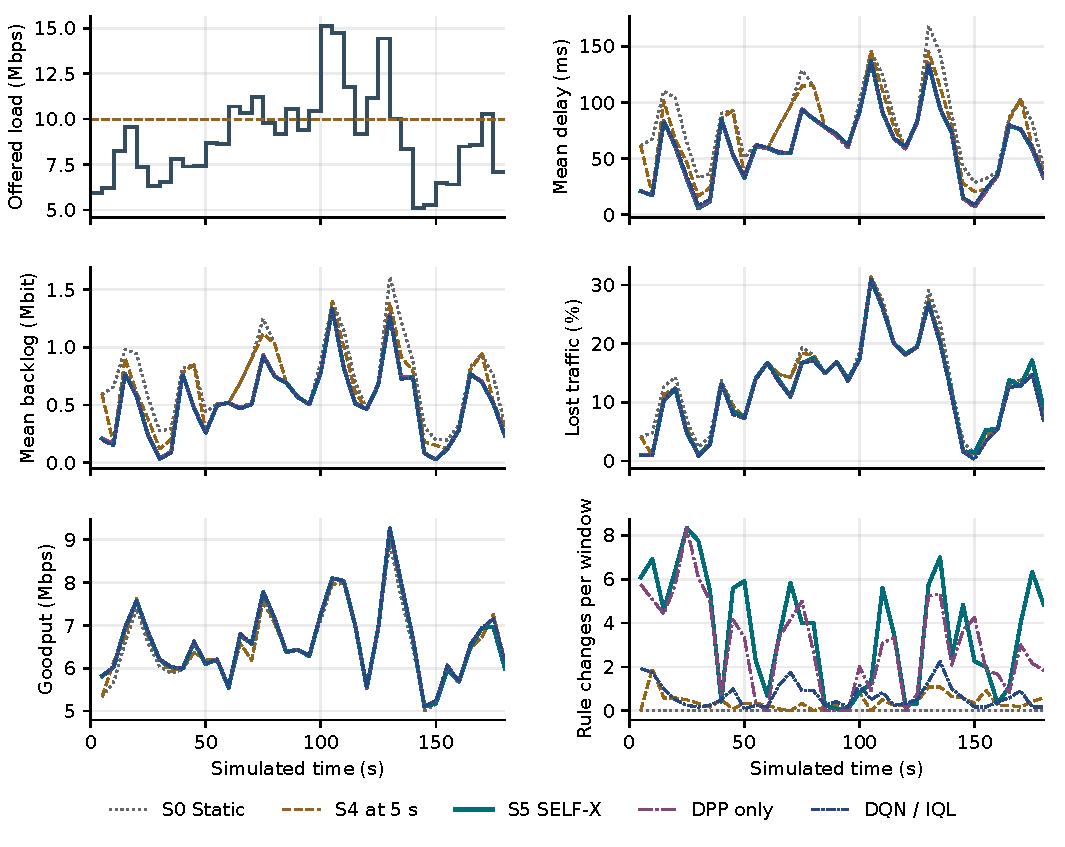
\includegraphics[width=.97\textwidth]{comparison/paper_window_traces.pdf}
\caption{Offered load, delay, mean backlog, traffic loss, goodput, and rule changes in aligned 5~s windows. Each point is the mean across the twelve test traces at that elapsed time. The dashed line in the offered-load panel marks the 10~Mbps capacity of one path. DQN and IQL share one curve because their effective actions coincide.}
\label{fig:windowtraces}
\end{figure*}

\subsection{Performance by workload}
Table~\ref{tab:profiles} shows absolute delay, loss, and goodput for the selected configurations within each synthetic profile. The absolute means complement the paired cadence estimates. Volatile traffic shows the largest delay gap between S4 and S5. In flash crowds, S5 lowers mean delay relative to S4 while losing more traffic. The profile effects are descriptive summaries over four paired traces each.

\begin{table}[t]
\centering
\caption{Mean Outcomes by Synthetic Workload}
\label{tab:profiles}
\footnotesize
\setlength{\tabcolsep}{3.2pt}
\begin{tabular}{@{}llrrr@{}}
\toprule
Workload & Arm & Delay (ms) & Loss (\%) & Mbps\\
\midrule
\ExpandedProfileRows
\bottomrule
\end{tabular}
\end{table}
